%\documentclass{article}[11pt]
\documentclass[varwidth,bib]{statapress}


\usepackage[crop,newcenter,frame]{pagedims}
\usepackage{sj-2}
\usepackage{epsfig}
\usepackage{stata}
\usepackage{shadow}
% EDITORS: volume number, issue number, month, and year
\sjsetissue{$vv$}{$ii$}{$mm$}{$yyyy$}

\usepackage{amsmath}
\usepackage{bbm}
\usepackage{amsfonts}
\usepackage{booktabs}
\usepackage{hyperref}
\usepackage{setspace}
\usepackage{soul}
\usepackage{lscape}
\usepackage{rotating}
\usepackage{multirow}
\usepackage{floatrow}
\usepackage{rotating,capt-of}
\usepackage{array}
\usepackage{subcaption}
%\usepackage[caption=false]{subfig}
\usepackage{bm}
\usepackage{bbm}
\usepackage{url}
\usepackage{color, colortbl}
\definecolor{Gray}{gray}{0.9}


\usepackage{amsthm}
\usepackage[stable]{footmisc}
\usepackage{graphicx}
\usepackage{booktabs}
\usepackage{longtable}
\usepackage{float}
\usepackage{subfloat}
\usepackage{verbatim}
\usepackage{caption}
\usepackage{fancyhdr}
\usepackage{algorithm}
\usepackage[noend]{algpseudocode}
%for algorithm
%\usepackage{algorithm}% http://ctan.org/pkg/algorithms
%\usepackage{algpseudocode}% http://ctan.org/pkg/algorithmicx
%\usepackage[ruled,vlined]{algorithm2e}

%to reference notes
\usepackage{cleveref}


\bibliographystyle{sj}
\hypersetup{
  colorlinks=true,
  linkcolor=blue,
  citecolor=blue,
  filecolor=blue,
  urlcolor=blue
}

%for arXiv
        \hypersetup{
           breaklinks=true,
           pdfusetitle=true, 
        }
        
\usepackage{natbib}

\DeclareMathOperator*{\argmin}{arg\,min}
\begin{document}

\inserttype[]{article}
\author{}{%
    Stefano DellaVigna \\ UC Berkeley \\  sdellavi@econ.berkeley.edu
\and
    Guido Imbens\\Graduate School of Business\\Stanford University \\ imbens@stanford.edu \vspace{4mm} \\ 
\and
    Woojin Kim \\ Stanford University \\ wjnkim@stanford.edu
\and
    David M. Ritzwoller \\ Stanford University \\ ritzwoll@stanford.edu
\and
    Damian Clarke\\Department of Economics \\ University of Chile \\ dclarke@fen.uchile.cl
\and
    Nicol\'as Par\'is\\Department of Economics \\ University of Chile \\ nparis@fen.uchile.cl
}
%TWO OPTIONS?  Second is riff on Cameron Miller piece
%\title[Inference with Spatial Dependence]{How to Conduct Inference with Spatial Dependence in Stata}
\title[Inference with Spatial Dependence]{A Practitioner's Guide to Inference with Spatial Dependence}
\maketitle

\begin{abstract}
  In many empirical applications in the social sciences, individuals-level observations interact or are subject to shared shocks across space.  In order to conduct valid statistical inference, such spatial dependence must be accounted for.  While a number of strategies to account for spatial dependence exist, these typically are based on strict assumptions about delimitation of dependence within certain geographic areas (\textit{i.e.}\ clustering), or modelling dependence solely in terms of distance.  In this paper, we discuss these common forms of inference with spatial dependence and their drawbacks, and introduce an alternative form of inference, laid out in \citet{Dellavignaetal2025}, known as Thresholding Multiple Outcomes (TMO).  This procedure for inference models dependence by using information from a range of variables to infer the dependence between units across space, and constructs standard errors and confidence intervals based on such dependence.  We introduce the command {\tt tmo}, which implements these procedures in Stata for a range of linear models including OLS and 2SLS. 
  \keywords{\inserttag spatial dependence, inference, multiple outcomes, standard errors.}
\end{abstract}


\clearpage
\section{Introduction}
Spatial dependence is a common feature of data in the social sciences.  Interactions between individuals in their neighbourhoods, cities, states or other social networks typically imply that individuals cannot be viewed as independent observations in space. And even absent direct interactions between individuals, shared underlying shocks typically occur in areas which are linked across potentially quite broad areas of space, and potentially in quite a complex fashion.  [INCLUDE EXAMPLES]

Such spatial dependence must be accounted for if one wishes to conduct inference on parameters estimated in econometric models.  Variance-covariance estimators in commonly estimated econometric models such as ordinary least squares (OLS) and two stage least squares (2SLS) typically start from the assumption of independence, but must be relaxed to account for more realistic interactions among observations across space. If such adjustments are not made, standard errors will be mis-estimated, generally resulting in standard errors which are too small, and confidence intervals which are too narrow.

In this paper we lay out considerations for conducting inference in models where spatial dependence among observations is suspected.  We discuss a number of existing common procedures and their limitations, and lay out a new procedure for inference with spatial correlation variance which leverages multiple outcome measures.  This procedure, referred to as Thresholding Multiple Outcomes (TMO) is described in \citet{Dellavignaetal2025} (and in this paper), and is accompanied by a Stata routine {\tt tmo} designed for a range of commonly encountered estimation methods in Stata which we document here.

Tools to relax the variance-covariance matrix in \textit{in certain ways} are default in many computational implementations in Stata.  For example, essentially all Stata estimators incorporate heteroscedasticity-robust estimators by default.  And similarly, cluster robust variance allows for \textit{limited} spatial dependence.  This ... \citet{Moulton1986,Moulton1990}.

However, this assumes a very specific form of dependence.  Additional forms of dependence can be explicitly based on distance or `economic distance'. \citet{Conley1999}
\citet{MullerWatson2022}
\citet{MullerWatson2022b}

It is reasonable, however, to ask what dependence looks like in practice.  This leads to a new way to estimate spatial dependence:
\citet{Dellavignaetal2025}.  Note that this considers inference on a parameter of interest.

To see what this looks like, consider a representative county.  Explain Figure \ref{fig:illustration}.

\begin{figure}[htpb!]
    \centering
    \caption{Spatial Standard Error Procedures}
    \label{fig:illustration}
    \begin{subfigure}{0.45\textwidth}
        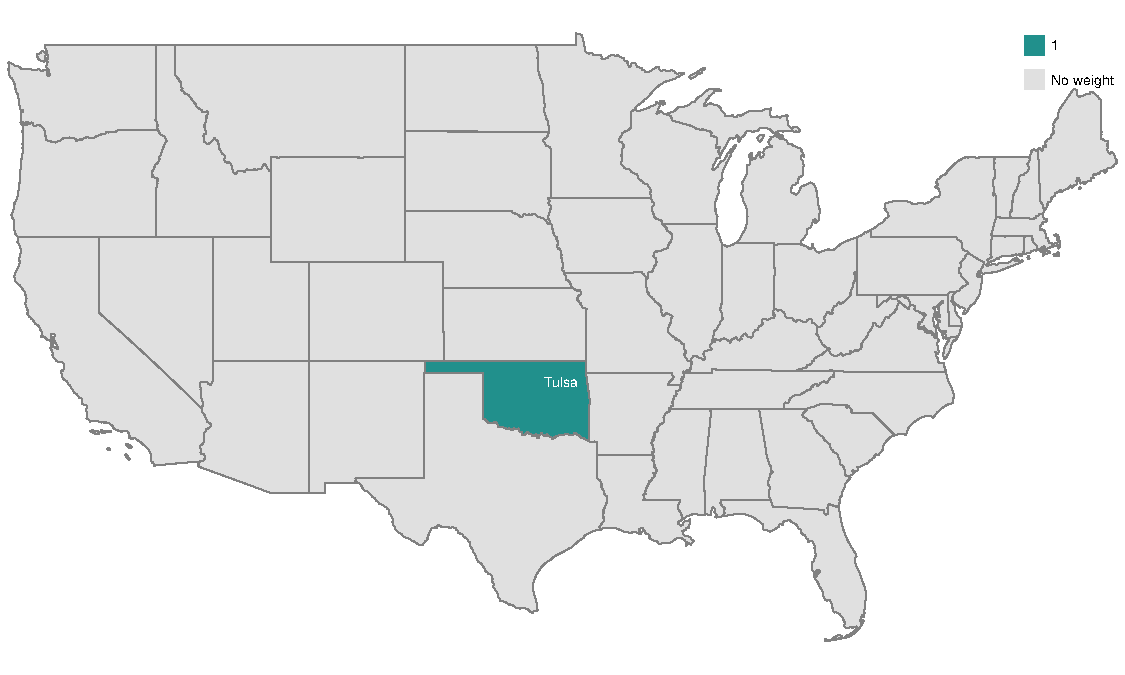
\includegraphics[width=\linewidth]{./figures/state_clustering.pdf}
      \caption{Clustering by State}
      \label{fig:cluster}
    \end{subfigure}
    \hfill
    \begin{subfigure}{0.45\textwidth}
      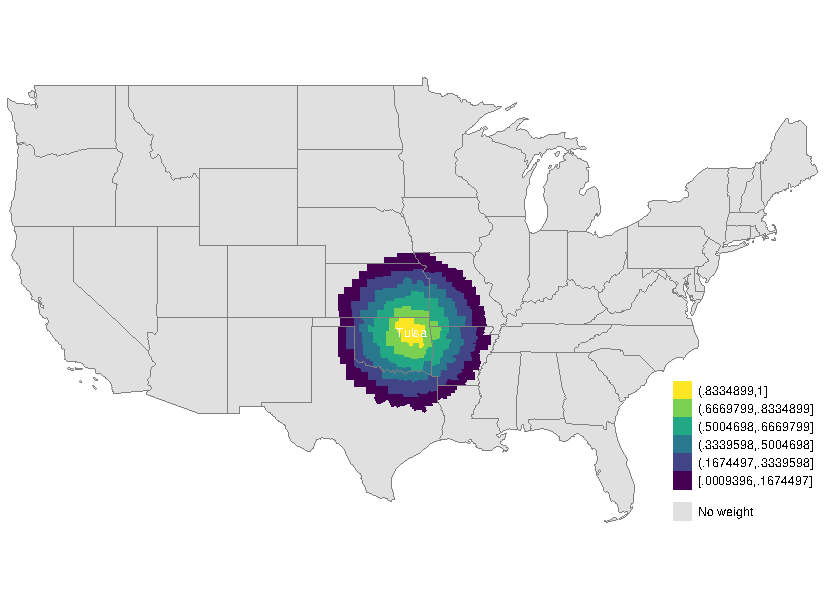
\includegraphics[width=\linewidth]{./figures/Conley.pdf}
      \caption{Conley}
      \label{fig:conley}
    \end{subfigure}

    \begin{subfigure}{0.45\textwidth}
        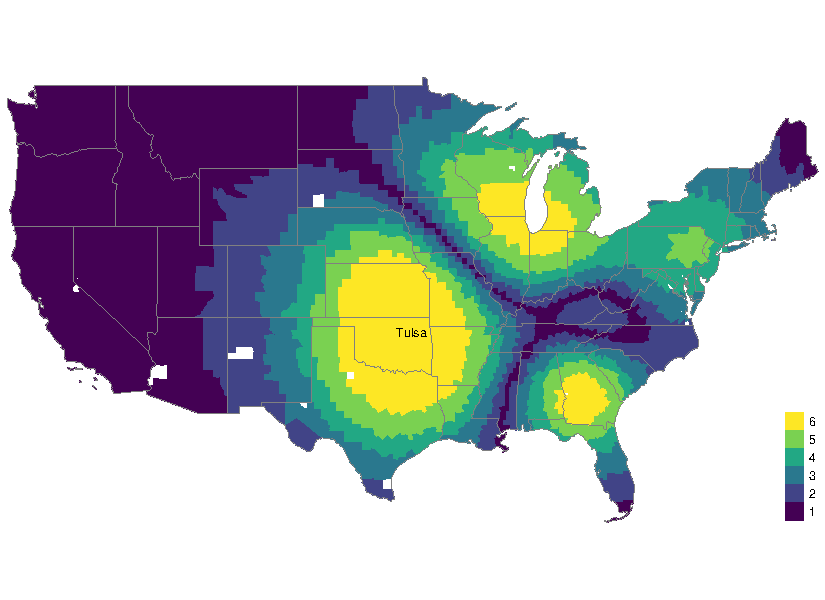
\includegraphics[width=\linewidth]{./figures/SCPC.pdf}
      \caption{SCPC}
      \label{fig:scpc}
    \end{subfigure}
    \hfill
    \begin{subfigure}{0.45\textwidth}
      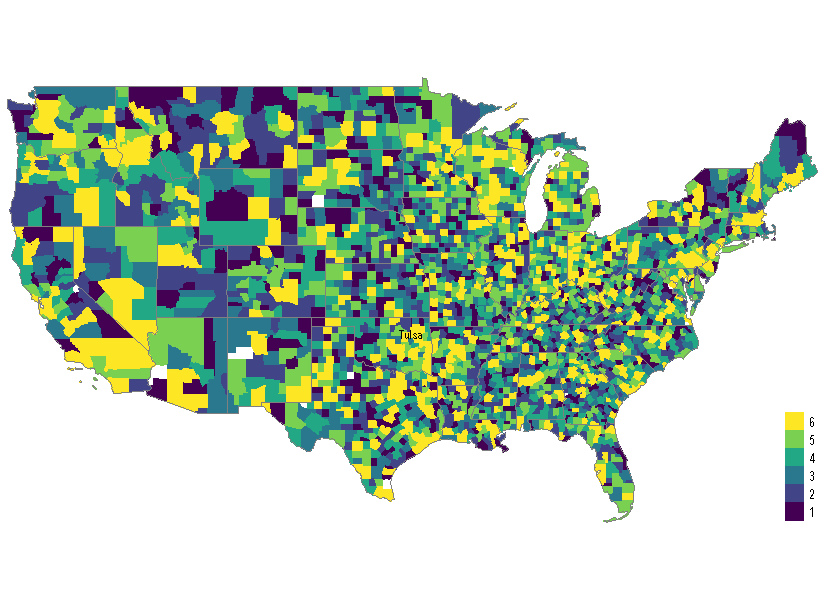
\includegraphics[width=\linewidth]{./figures/tmo.pdf}
      \caption{TMO}
      \label{fig:tmo}
    \end{subfigure}
  \end{figure}

In this paper we ... Primer on estimating standard errors with spatial dependence in Stata.  Introduce TMO.  Discuss a number of key outcomes in US case.  

Other spatial tools in Stata include...

In what remains of this paper, we begin by describing methods in Section \ref{scn:methods}, first discussing proposals to deal with spatial dependence, before focusing on TMO more generally.  We discuss a Stata command to implement TMO in Section \ref{scn:command}, before documenting a number of examples of the use of this command---{\tt tmo}---in Section \ref{scn:examples}.  Section \ref{scn:discussion} lays out key points of relevance for practitioners and concludes.

\section{Methods}
\label{scn:methods}
\subsection{A Simple Bivariate Regression Model}
Consider estimating a simple bivariate regression model of the type:
\begin{equation}
\label{eqn:linmodel}
Y_{i}=\alpha+\tau W_i + \varepsilon_i,
\end{equation}
based on a sample of data $i=1,\ldots, N$, where $Y_i$ is some outcome of interest, $W_i$ some treatment or independent variable of interest and $\varepsilon_i$ an unobserved term.  Assume now that $\mathbb{E}[\varepsilon_i|W_i]=0$. In this setting, the parameters $\alpha$ and $\tau$ can be estimated consistently by ordinary least squares, and denoted $\widehat\alpha$ and $\widehat\tau$ respectively.  Here---and in most empirical settings---we are most interested in the quantity $\widehat\tau$.

While the estimation of $\widehat\tau$ is straightforward, the estimation of the standard error for this estimate hinges upon assumptions about the correlation among residuals $\varepsilon_i$ within the sample.  To see this, note that the standard error is the square root of the following variance term:
\begin{equation}
\mathbb{V}(\widehat\tau|W)=(W^\prime W)^{-1}W^\prime\Omega W(W^\prime W)^{-1}.
\end{equation}
This depends, crucially, on the matrix $\Omega$ which is an $N\times N$ matrix describing the covariance between each $\varepsilon_i$ in the sample.  The most restrictive assumption about this matrix is that all observations share a common variance, and all observations are independent, or in other words, observations are independent and identically distributed.  In this case, $\Omega$ simplifies to $\sigma^2 I$, with $\sigma^2$ referring to the variance of $Y_i$, and $I$ and $N\times N$ identity matrix.  This leads to the simple variance expression:
\begin{equation}
\label{eqn:VarOLS}
\mathbb{V}(\widehat\tau|W)=\sigma^2(W^\prime W)^{-1},
\end{equation}
which is returned as default in computational estimators of \eqref{eqn:linmodel}.

The assumption of a common variance can be loosened quite simply to reflect heteroscedasticity, as laid out in seminal work of \citet{Huber1967,Eicker1967,white80}.  In this case, rather than \eqref{eqn:VarOLS}, the heteroscedasticity-robust analogue:
\begin{equation}
\label{eqn:VarHR}
\widehat{\mathbb{V}}(\widehat\tau \mid W)_H = (W^\prime W)^{-1} \left( \sum_{i=1}^N \widehat\varepsilon_i^2 W_i W_i^\prime \right) (W^\prime W)^{-1}
\end{equation}
can be estimated, where $\widehat\varepsilon_i=Y_i-\widehat\alpha-\widehat\tau W_i$.  Again, such a variance estimator is standard in most computational implementations of regression estimators, such as Stata's {\tt robust} option.\footnote{In practice, because of finite sample biases in this estimator, most software packages report finite-sample corrected versions of the heteroscedasticity-robust variance estimator. Stata's {\tt robust} option reports the HC1 estimator by default, which rescales the HC0 matrix in \eqref{eqn:VarHR} by $\tfrac{N}{N-k}$, where $k$ is the number of estimated parameters (2 in this case).  Other common variants include HC2 and HC3, which apply leverage-based corrections to adjust for influential observations \citep[see e.g.][]{MackinnonWhite1985,LongErwin2000}, also available via Stata's {vce()} option.}  However, both \eqref{eqn:VarOLS} and \eqref{eqn:VarHR} are predicated on the assumption that observations are independent, and as such $\varepsilon_i$ and $\varepsilon_j$ are not correlated for all observation pairs $i$ and $j$ where $i\neq j$.   In many cases, this is likely viewed as an unrealistic assumption, and instead some sort of spatial (or other) correlation is presumed to exist between terms $\varepsilon_i$ and $\varepsilon_j$.  In this case, a number of procedures exist to seek to conduct appropriate inference despite such dependence.

\subsubsection{Restricting Elements of $\Omega$}
A first way to proceed is to note that we can permit limited sorts of spatial dependence by clustering at some aggregate geographic level.  This recognises the importance of intra-group clustering \citep{Moulton1986}, by allowing certain dependence across space within $\Omega$ while restricting elements of $\Omega$ outside of any specific cluster to be 0. In essence, this allows arbitrary correlations within some specific geographical or other boundary, while restricting any dependence across clusters.  Such a case can be viewed schematically in $\Omega_{CR}$ below, for a cluster-robust case assuming a number of blocks, compared to the more restrictive heteroscedasticity-robust option $\Omega_H$.
\[
\Omega_{\text{CR}} =
\begin{bmatrix}
\varepsilon_1^2 & \varepsilon_1 \varepsilon_2 & 0 & 0 & \cdots & 0 & 0 \\
\varepsilon_2 \varepsilon_1 & \varepsilon_2^2 & 0 & 0 & \cdots & 0 & 0 \\
0 & 0 & \varepsilon_3^2 & \varepsilon_3 \varepsilon_4 & \cdots & 0 & 0 \\
0 & 0 & \varepsilon_4 \varepsilon_3 & \varepsilon_4^2 & \cdots & 0 & 0 \\
\vdots & \vdots & \vdots & \vdots & \ddots & \vdots & \vdots \\
0 & 0 & 0 & 0 & \cdots & \varepsilon_{N-1}^2 & \varepsilon_{N-1} \varepsilon_{N} \\
0 & 0 & 0 & 0 & \cdots & \varepsilon_N \varepsilon_{N-1} & \varepsilon_N^2 \\
\end{bmatrix}
\Omega_{\text{H}} =
\begin{bmatrix}
\sigma_1^2 & 0 & \cdots & 0 \\
0 & \sigma_2^2 & \cdots & 0 \\
\vdots & \vdots & \ddots & \vdots \\
0 & 0 & \cdots & \sigma_N^2
\end{bmatrix}
\]

Inference based on clustering is standard, following \citet{LiangZeger1986,MackinnonWhite1985}, 
\begin{equation}
\label{eqn:VarCR}
\widehat{\mathbb{V}}(\widehat\tau \mid W)_{CR} = (W^\prime W)^{-1} \left( \sum_{g=1}^G W_g^\prime \widehat\varepsilon_g \widehat\varepsilon_g^\prime W_g \right) (W^\prime W)^{-1}
\end{equation}
where the $g$ refers to each of the $G$ clusters, $\widehat\varepsilon_g$ a vector of residuals for each cluster,  In practice, Stata's implementation of such cluster-robust variance estimates incorporates a finite sample correction factor, multiplying \eqref{eqn:VarCR} by $\frac{G}{G-1}\frac{N-1}{N-K}$ to correct for the downward bias in standard errors when the number of clusters is small \citep{CameronMiller2015,Rogers1993}.


\subsubsection{Distance-based limiting}
A drawback of such an approach is that spatial dependence is viewed as being sharply demarcated by the borders or limits of clusters.  Another common alternative which seeks to avoid such sharp demarcation at geographic borders instead views spatial dependence in terms of distance.  This approach, proposed by \citet{Conley1999}, allows for residual dependence to decay continuously over space. Rather than imposing a block-diagonal structure in $\Omega$, Conley's estimator permits non-zero covariances between all observations but downweights them by a kernel function of geographic distance, up to some maximum point at which case zero covariance is assumed.

Formally, the Conley variance estimator takes the form:
\begin{equation}
\label{eqn:VarConley}
\widehat{\mathbb{V}}(\widehat\tau \mid W)_{\text{Conley}} = (W^\prime W)^{-1} \left( \sum_{i=1}^N \sum_{j=1}^N K_{ij} \widehat\varepsilon_i \widehat\varepsilon_j W_i W_j^\prime \right) (W^\prime W)^{-1},
\end{equation}
where $K_{ij}=K(d_{ij}/b)$ is a kernel function of the distance $d_{ij}$ between units $i$ and $j$, and $b$ is a bandwidth parameter. Typical choices for $K(\cdot)$ include the Bartlett or uniform kernel.\footnote{These are defined respectively as $K(d_{ij}/b) = 1 - d_{ij}/b$ for $d_{ij} \leq b$ and $0$ otherwise, which applies linearly decreasing weights as distance increases; and $K(d_{ij}/b) = \mathbbm{1}\{d_{ij} \leq b\}$, which applies equal weight to all pairs within a cutoff distance $b$.} Intuitively, this estimator treats spatial correlation as strongest between nearby units, either uniformly, or declining smoothly with distance, and ultimately reaching zero beyond a certain cutoff.  We can see intuitively that as $K_{ij}$ decays to zero, the correlation between residuals in \eqref{eqn:VarConley} becomes irrelevant in the variance estimate, as the summation term resolves to 0 when $K_{ij}=0$.

There are also alternative approaches which seek to take such-distance based approaches.  \citet{MullerWatson2022} point out that if observations are not uniform in space, then methods such as \eqref{eqn:VarConley} will not be asymptotically valid, and potentially suffer from size distortions in finite samples which lead to over-rejection of null hypotheses.  Thus, this leads to suggestions as laid out in  \citet{MullerWatson2022,MullerWatson2022b} in which rather than using kernel functions to model the location of units across space, the location of units is modelled based on principal components which capture spatial agglomeration.  They show that this approach offers improved performance in cases where spatial agglomeration of observations occurs, and, when confidence intervals are constructed based on critical values which consider such spatial dependence, can result in large improvements in error rates \citep{MullerWatson2022b}.

\subsubsection{Thresholding Multiple Outcomes}
\paragraph{Using Multiple Outcomes to Infer Cross-Space Correlations} 
Ultimately, however, both cluster-robust and distance-based procedures are limiting, either by assuming a strict off-diagonal zero correlation, or by assuming a zero correlation among units beyond some specified cut-off point.  This limitation occurs given that these approaches are based entirely upon modelling spatial correlations by considering how \textit{units} relate across space, rather than considering how outcomes $Y_i$ themselves relate across space.  Thus, a more realistic approach may be to seek to infer geographic dependence by examining the correlation of a range of actual measures over space.  

To this end, \citet{Dellavignaetal2025} introduce Thresholding Multiple Outcomes, or TMO, in which auxiliary measures are used to determine whether correlations exist between particular locations in data.  This requires information on a number $d$ of auxiliary outcomes, which we will denote $Y_i^{(1)}, \ldots, Y_i^{(d)}$.  If such multiple alternative outcomes exist, we can use these measures to assess whether systematic correlation exists between residuals over space.

Namely, each of these outcomes which we will generically refer to as $Y_i^{(j)}$ can themselves be regressed on our outcome of interest in \eqref{eqn:linmodel}.  The residual term from this regression is denoted $\widehat\varepsilon_i^{(j)}$, and this can be normalised to have a variance of 1 as $\tilde\varepsilon_i^{(j)}=\widehat\varepsilon_i^{(j)}/\sqrt{\frac{1}{N}(\widehat\varepsilon_i^{(j)})^2}$.  We will seek to leverage these residuals to determine the correlation of outcomes between locations across space.  To do so, the covariance and the correlation between residuals for some locations $i$ and $i^\prime$ are denoted:
\begin{equation}
\widehat\lambda_{i,i^\prime}=\frac{1}{d}\sum_{j=1}^d(\tilde\varepsilon_i^{(j)}-\bar{\varepsilon_i})(\tilde\varepsilon_{i^\prime}^{(j)}-\bar{\varepsilon_{i^\prime}}) \qquad \text{and} \qquad \widehat\rho_{i,i^\prime}=\frac{\widehat\lambda_{i,i^\prime}}{\sqrt{\widehat\lambda_{i,i}\widehat\lambda_{i^\prime,i^\prime}}},
\end{equation}
where $\bar{\varepsilon_i}=\frac{1}{d}\sum_{j=1}^d\tilde\varepsilon_i^{(j)}$. This quantity $\widehat\rho_{i,i^\prime}$ is of key importance, as it summaries, across all outcomes $d$, the tendency of residuals from observation $i$ and $i^\prime$ to be correlated.

The logic of TMO is that while most pairs of units are not correlated, some will be, and the correlation between auxiliary outcomes $\widehat\rho_{i,i^\prime}$ can be used to determine those observations which are correlated across space.  Specifically, setting some threshold value $\delta$ as the value above which observations are inferred to be meaningfully correlated, we can write $\widehat\Omega$ as:
\[
\widehat\Omega = 
\begin{cases}
  \widehat\varepsilon_i^{0}\widehat\varepsilon_i^{0} & \text{if } i=i^\prime, \\
  \widehat\varepsilon_i^{0}\widehat\varepsilon_{i^\prime}^{0} & \text{if } \widehat\rho_{i,i^\prime}\geq\delta, \\
  0 & \text{if } \widehat\rho_{i,i^\prime}<\delta.
\end{cases}
\]
In essence, this threshold term $\delta$ is used to indicate which units have a systematic correlation between residuals across space, and as such account for this correlation in variance estimates.  Note that previously, off diagonal terms were $\widehat\varepsilon_i^{0}\widehat\varepsilon_{i^\prime}^{0}$ were allowed to be non-zero if they fulfilled specific \textit{geographic} criteria such as sharing a cluster, whereas here with the incorporation of $\delta$, these terms are allowed to be non-zero if \textit{auxiliary outcomes themselves} are observed to be correlated across space.

\citet{Dellavignaetal2025} show that under two assumptions, these procedures result in a consistent variance estimate.  Specifically, these assumptions are referred to as `proportionality' and `sparsity'.  The first of these implies that the covariance of residuals for auxiliary outcomes is informative of the correlation across residuals for the outcome of interest.  And the second assumption implies that there is some limit on the number of units which are actually correlated with any other unit. 

\paragraph{Determining Thresholds for Cross-Space Correlations} Provided that such assumptions are reasonable, the remaining question is what threshold value for $\delta$ should be used as a threshold for determining correlations.  In effect, most pairs of observations will not be correlated (``null pairs''), while some small proportion (``non-nulls'') will be correlated.  Selecting a threshold thus can be viewed as a trade-off between potentially excluding relevant non-nulls (which will understate the variance) and including irrelevant nulls (which will overstate the variance). \citet{Dellavignaetal2025} propose determining the optimal threshold $\delta^\star$ as the value which sets the proportion of misclassification among pairs flagged as being `non-null' at 50\%.  This is a False Discovery Rate (FDR), and implies that if $\delta^{\star}$ were lowered, more than half of the pairs added would actually be null, whereas if $\delta^\star$ were increased, more than half of the pairs removed would actually be non-null.  %Heuristically, the idea behind this threshold selection is that most pairs of outcomes will not be correlated over space, 

Empirically, the value $\delta^\star$ is determined with this trade-off in mind.  In order to resolve this trade-off, we define as $F_0(\cdot)$ the (unknown) distribution function of empirical correlations $\widehat\rho_{i,i^\prime}$ for \textbf{null} pairs of units (we discuss the estimation of this below).  Similarly, we can define $F^+_0(\cdot)\equiv2(1-F_0(\cdot))$ as the right distribution for the \textit{absolute} correlations $\lvert\widehat\rho_{i,i^\prime}\rvert$.\footnote{Could point to an appendix where we simulate an example and show this in a step-by-step way so readers can easily understand the mechanics...?}  Similarly, we denote as $F^+(\delta)=\Pr(\lvert\widehat\rho_{i,i^\prime}\rvert\geq\delta)$ the right distribution function for absolute correlations for both null and non-null pairs of units (\textit{i.e.} the unconditional distribution). 

We can write the probability that observations whose $\widehat\rho_{i,i^\prime}\geq\delta$ are non-null and null as follows for a specific threshold choice $\delta$:
\begin{equation}
\Pr(\text{Non-Null}\big|\ \lvert\widehat\rho_{i,i^\prime}\rvert\geq\delta) = \frac{F^+(\delta)-p_0F_0^+(\delta)}{F^+(\delta)} \qquad \Pr(\text{Null}\big|\ \lvert\widehat\rho_{i,i^\prime}\rvert\geq\delta) = \frac{p_0F_0^+(\delta)}{F^+(\delta)},
\end{equation}
where $p_0$ refers to the proportion of pairs of units with a null relationship across space.  We can then take the difference between the probability of observations being null and non-null as proportional to the following:
\begin{equation}
Q(\delta)=(F^+(\delta)-p_0F_0^+(\delta))-p_0F_0^+(\delta) = F^+(\delta)-2p_0F_0^+(\delta).
\end{equation}
A key property to note with $Q(\delta)$ is that this will be increasing in $\delta$ if more nulls are admitted than non-nulls, and decreasing in $\delta$ if more non-nulls are admitted than nulls.  Thus, maximizing $Q(\delta)$ with respects to $\delta$ finds the point at which half the added pairs are null, and half are non-null.

This suggests an (infeasible) criteria to select delta as maximizing the following quantity $\widetilde{Q}$:
\begin{equation}
\widetilde{Q}_{N,d}(\delta)=\widehat{F}^+(\delta)-2p_0F_0^+(\delta) \qquad \text{where } \widehat{F}^+(\delta)=\frac{2}{N(N-1)}\sum_{i=1}^N\sum_{i^\prime<i}\mathbbm{1}\{\lvert\widehat\rho_{i,i^\prime}\rvert>\delta\}.
\end{equation}
This quantity cannot yet be estimated for two reasons.  Firstly,  while the distribution of both null and non-null pairs can be estimated from data as $\widehat{F}^+(\delta)$, the distribution of just null pairs $\widehat{F}_0^+(\delta)$ is unknown.  And secondly, the proportion of nulls themselves ($p_0$) is also unknown.  In line with the sparsity assumption, the quantity $p_0$ can (conservatively) be set equal to 1.  This leads to a feasible criteria: 
\begin{equation}
\label{eqn:objQ}
\widehat{Q}_{N,d}(\delta)=\widehat{F}^+(\delta)-2F_0^+(\delta),
\end{equation}
where the optimal threshold $\delta^\star$ is chosen as the quantity that maximizes \eqref{eqn:objQ}.

Thus, a final step required to actually estimate $\widehat{Q}_{N,d}$ is to estimate the null distribution $F_0(\cdot)$.  This cannot be estimated directly as the distribution of $\widehat\rho_{i,i^\prime}$ given that this distribution will contain both null and non-null pairs.  However, given that most pairs are assumed to actually be null pairs, this leads to the proposal in \citet{Dellavignaetal2025} to estimate this null distribution by fitting a Normal distribution to the central part of the empirical distribution of $\widehat\rho_{i,i^\prime}$ which will overwhelmingly consist of null pairs.  In the interests of completion, if $\Phi_v(\cdot)$ refers to the normal distribution with variance $v$, and $\Phi^{-1}_v(\cdot)$ its inverse, then the interquartile function can be written as $IQR_{v,0}=\Phi^{-1}_v(0.75)-\Phi^{-1}_v(0.25)$. Similarly, defining the empirical distribution of observed correlations as:
\[
G_{N,d}(\delta)=\frac{2}{N(N-1)}\sum_{i=1}^N\sum_{i^\prime<i}\mathbbm{1}\{\widehat\rho_{i,i^\prime}<\delta\},
\]
we can define the inverse and interquartile range of observed correlations (respectively) as $G^{-1}_{N,d}(\cdot)$ and $\widehat{IQR}=G^{-1}_{N,d}(0.75)-G^{-1}_{N,d}(0.25)$.  The distribution $F^+_0$ is thus estimated by setting $v$ to the quantity which resolves $IQR_{\widehat{v},0}=\widehat{IQR}$.

%TMO adjusts standard errors in settings with spatial dependence without modeling a full covariance structure. Start from your main outcome $Y_i^{(0)}$ and a set of auxiliary outcomes $Y_i^{(1)}$,$\ldots,Y_i^{(d)}$. For each outcome, regress on $W_i$ and compute normalized residuals. The key assumption is that the spatial correlation in the residuals of $Y_i^{(0)}$ is mirrored in those of the auxiliaries. Using the auxiliaries, estimate pairwise correlations across locations and, by comparing their empirical distribution to a null benchmark, choose a threshold $\hat\delta$ that flags ``highly correlated'' pairs.

%Then build $\hat\Sigma^{(0)}(\hat\delta)$: keep the product of residuals for $Y_i^{(0)}$ on the diagonal and for off-diagonal entries only when $|\hat\rho_{i,i’}|\ge \hat\delta^*$. Plug this into the sandwich formula, to obtain spatially robust standard errors.

At the beginning of Section \ref{scn:examples} we will examine an empirical example which steps through each of these steps, in essence considering the estimation of $\widehat\rho_{i,i^\prime}$, $G_{N,d}(\delta)$, $\widehat{v}$, and $\delta^\star$, and resultingly, the standard errors and confidence intervals corresponding to our regression estimate of interest $\widehat\tau$.  Examining this in practice helps to elucidate the steps in both thresholding, and estimating cross-space correlations.  A summarised statement of the entire estimation algorithm as defined in \citet{Dellavignaetal2025} is provided as
Algorithm \ref{alg:TMP} in an Appendix to this article.

\subsection{Alternative Estimators}
While the above treatment begins with a bivariate linear regression model in \eqref{eqn:linmodel}, the above procedures can quite simply be ...


\subsection{Combining TMO with Distance-Based Procedures}



 \clearpage
\section{The {\tt tmo} command}
\label{scn:command}
\subsection{Syntax}
The {\tt tmo} command is an e-class command with the following syntax:
\begin{stsyntax}
\/
tmo, cmd({\it cmdline\/}) 
x(\dunderbar{\it varname}) ylist(\dunderbar{\it varlist}) \dunderbar{i}dvar(\dunderbar{\it varname}) \optional{\dunderbar{options}}
\end{stsyntax}
\subsection{Options}

\noindent {\tt cmd(\it cmdline\rm )} \it cmdline\rm\ is the command that produces the regression of interest. \rm tmo currently supports regressions using \dunderbar{\tt regress}, \dunderbar{\tt areg}, \dunderbar{\tt reghdfe}, \dunderbar{\tt ivregress}, \dunderbar{\tt ivreg2}, or \dunderbar{\tt ivreghdfe}.

\noindent {\tt x(\dunderbar{\it varname})} Regressor of interest in \tt cmd \rm for which to estimate TMO standard errors. \rm tmo \it estimates the standard error for only this declared independent variable.

\noindent {\tt ylist(\dunderbar{\it varlist})} List of auxiliary outcomes to use in \rm tmo.

\noindent {\tt \dunderbar{i}dvar(\dunderbar{\it varname})} Location identifier variable; must be unique (within each time period for panel case).

\noindent {\tt misslimit(\it \#\rm )} Limit for proportion of observations allowed to be missing for auxiliary outcomes. Auxiliary outcomes missing more than \tt misslimit \rm are not used. Must be between [0,1]; default is 0.1.

\subsubsection*{Panel Setting}
{\tt timevar(\dunderbar{\it varname})} Time identifier variable; must be declared for panel case.

\subsubsection*{Distance-based Settings}
\noindent {\tt latitude(\dunderbar{\it varname})} Latitude variable in signed decimal degrees.

\noindent {\tt longitude(\dunderbar{\it varname})} Longitude variable in signed decimal degrees.

{\tt distthreshold(\it \#\rm )} Distance threshold to allow for arbitrary correlation between pairs of locations that are \tt distthreshold \rm or closer. Distances are measured in kilometres by default; see the {\tt miles} option. Combines \rm tmo \it with a Conley adjustment using a uniform kernel (but see \rm {\tt distkernel()}\it). Requires \tt latitude \rm and \tt longitude.

\noindent {\tt miles} Measure distances for {\tt distthreshold()} in miles rather than kilometres.

\noindent {\tt distkernel(\it str\rm )} Kernel for the distance-based adjustment; either {\tt uniform} (the default: pairs within {\tt distthreshold()} receive full weight) or {\tt bartlett} (pairs not selected by the TMO threshold receive weight $1-d_{ii^\prime}/b$, declining linearly to zero at the cutoff $b$, analogous to the pair-level SCPC combination). Requires {\tt distthreshold()}; may not be combined with {\tt scpc\_cmd()}.

\subsubsection*{Saving Figures and Tables}
{\tt filesuffix(\it str\rm )} Folder path and base filename for saving figures and results. Required for \tt plot \rm or \tt save \rm options.

\noindent {\tt savedyad} Save Stata data file with correlation and contribution to standard error for each location pair.

\noindent {\tt plotq} Save plot of optimal threshold estimator.

\noindent {\tt plothist} Save plot for histogram of correlations between locations.

\noindent {\tt plothistnbins(\it \#\rm )} Number of bins for histogram of correlations (default 10000).

\noindent {\tt plotse} Save plot for standard error estimates across thresholds.

\noindent {\tt saveplotseest} Save Stata data file with standard error estimates across thresholds.

\noindent {\tt saveest} Save results in \tt r() \rm to Stata data file.

\subsubsection*{Custom Threshold}
{\tt threshold(\it \#\rm )} Set custom threshold instead of using the optimal threshold from the interquartile range method. Must be between [0,1].

\noindent {\tt thresholdoff} Turns off the \rm tmo \it adjustment entirely.

\subsubsection*{SCPC Options}
{\tt scpc\_cmd ({\it cmdline}\rm)} \rm Command for regression of interest before applying SCPC adjustment. Combines \rm tmo  with the SCPC method from \citet{MullerWatson2022}: pairs selected by the TMO threshold enter the variance with their raw covariance, while all remaining pairs enter through the implicit SCPC kernel weight. Requires \tt latitude \rm and \tt longitude\rm.

\noindent {\tt scpc\_uncond} Turns on the unconditional SCPC inference setting.
\subsubsection{Returned Objects}
\texttt{tmo} is an e-class command, and stores the following in \texttt{e()}:

\noindent Scalars:

\begin{tabular}{lp{9.5cm}}
  \texttt{e(beta)}              & point estimate for the variable declared in {\tt x()} \\
  \texttt{e(orig\_se)}          & standard error from the original command in {\tt cmd()} \\
  \texttt{e(tmo\_se)}           & TMO-adjusted standard error \\
  \texttt{e(lb)}, \texttt{e(ub)} & bounds of the TMO-adjusted 95\% confidence interval \\
  \texttt{e(threshold)}         & optimal (or user-set) threshold $\hat\delta$ \\
  \texttt{e(pct\_ge\_thres)}    & \% of off-diagonal pairs included in the variance \\
  \texttt{e(pct\_ge\_thres\_nocl)} & \% of pairs over the threshold outside clusters/Conley \\
  \texttt{e(N)}, \texttt{e(N\_loc)}, \texttt{e(N\_clust)} & observations, locations, and clusters \\
  \texttt{e(T)}                 & time periods (panel case) \\
  \texttt{e(N\_outcomes)}       & number of auxiliary outcomes used \\
  \texttt{e(dof)}               & degrees of freedom of the fitted null distribution \\
  \texttt{e(finite\_sample\_dof)} & finite-sample degrees-of-freedom adjustment \\
  \texttt{e(df\_r)}             & residual degrees of freedom \\
  \texttt{e(r2)}, \texttt{e(r2\_a)}, \texttt{e(rmse)} & fit statistics from the original command \\
  \texttt{e(scpc\_cv)}          & SCPC critical value (when {\tt scpc\_cmd()} is used) \\
\end{tabular}

\vspace{3mm}
\noindent Matrices:

\vspace{1mm}
\noindent
The matrices {\tt e(b)} and {\tt e(V)} contain the point estimate and TMO-adjusted variance for the variable declared in {\tt x()}, facilitating the exportation of results with routines such as {\tt estout}.



\section{Examples}
\label{scn:examples}
\subsection{An Illustrative Example: OLS and US counties}
It is illustrative to view the principles of TMO in a specific empirical setting.  To do so we will consider an example from \citet{Dellavignaetal2025} in which data on county-level outcomes in the USA have been collated.  In particular, consider the model where yyyy is regression on xxxxx, along with state fixed effects.  Below we load...   


%Let's explain what we're doing here (eg walk readers through the variables). Point to these data as bundled with the routine.  Show graph with coverage by state over time for an appendix (https://www.jstatsoft.org/article/view/v107i07/4504)?

  \begin{stlog}
    . tmo, cmd(reg PIN_persincpc_d EDU_college_d i.stfips, r) x(EDU_college_d) ///
>     ylist(`ylist') i(fips) plothist plotq file("figures/")
file{\bftt{ figures/_qt.pdf}} saved as PDF format
file {\bftt{figures/_hist.png}} written in PNG format
{\smallskip}
Linear Regression with TMO                              Number of obs =  3,060
                                                        R-squared     = 0.3434
                                                        Adj R-squared = 0.3434
                                                        Root MSE      = 0.1409
{\smallskip}
\HLI{13}{\TOPT}\HLI{64}
PIN_persin{\tytilde}d {\VBAR} Coefficient  Std. err.      t    P>|t|     [95\% conf. interval]
\HLI{13}{\PLUS}\HLI{64}
EDU_colleg{\tytilde}d {\VBAR}   .1745893   .0197081     8.86   0.000     .1359466     .213232
\HLI{13}{\BOTT}\HLI{64}
\HLI{79}
                                                                               
                                                   Optimal threshold      0.389
                                            \% of off-diag in SE est.      0.497
                              \% >= threshold (excl. clusters/Conley)      0.497
                                                          \# outcomes     90.000
                                                  Degrees of freedom     59.986
\HLI{79}

  \end{stlog}


The upper panel reports the conventional OLS results. The lower block summarizes the TMO adjustment. The \textit{Optimal threshold} $\hat\delta$ is a data–driven cutoff for the absolute Fisher–$z$ correlations across locations; pairs with $|\hat\rho_{i,i'}|\ge\hat\delta$ are treated as correlated when constructing $\widehat{\Sigma}^{(0)}(\hat\delta)$. From all the pairs 49\% reports the share of off–diagonal entries retained by this rule, and thus the extent of cross–location dependence incorporated in the variance. When TMO augments clustering or Conley, that records has the additional pairs contributed by TMO beyond the baseline method. In this case we used 90 auxiliary outcomes used to learn the correlation structure, finally the degrees of freedom reports the width of the normal reference used to set $\hat\delta$ (estimated from the interquartile range of Fisher–$z$ correlations).

The figures document the choice of $\hat\delta$. Figure~\ref{fisherCorr} shows the empirical distribution of Fisher–$z$ correlations across locations together with the fitted $N(0,\hat v)$ reference; the dashed vertical lines at $\pm\hat\delta$ indicate which pairs populate the off–diagonal of $\widehat{\Sigma}^{(0)}(\hat\delta)$. Figure~\ref{opThreshol} then plots the threshold objective $\hat Q_{n,d}(\delta)$; the dashed line marks its maximizer at $\hat\delta$ (larger $\delta$ yields a more conservative selection of pairs). The reported standard error is computed as $(W^\top W)^{-1}\!\bigl(W^\top \widehat{\Sigma}^{(0)}(\hat\delta) W\bigr)(W^\top W)^{-1}$.
  \begin{figure}[H]
    \caption{Correlations between residuals across US counties}
    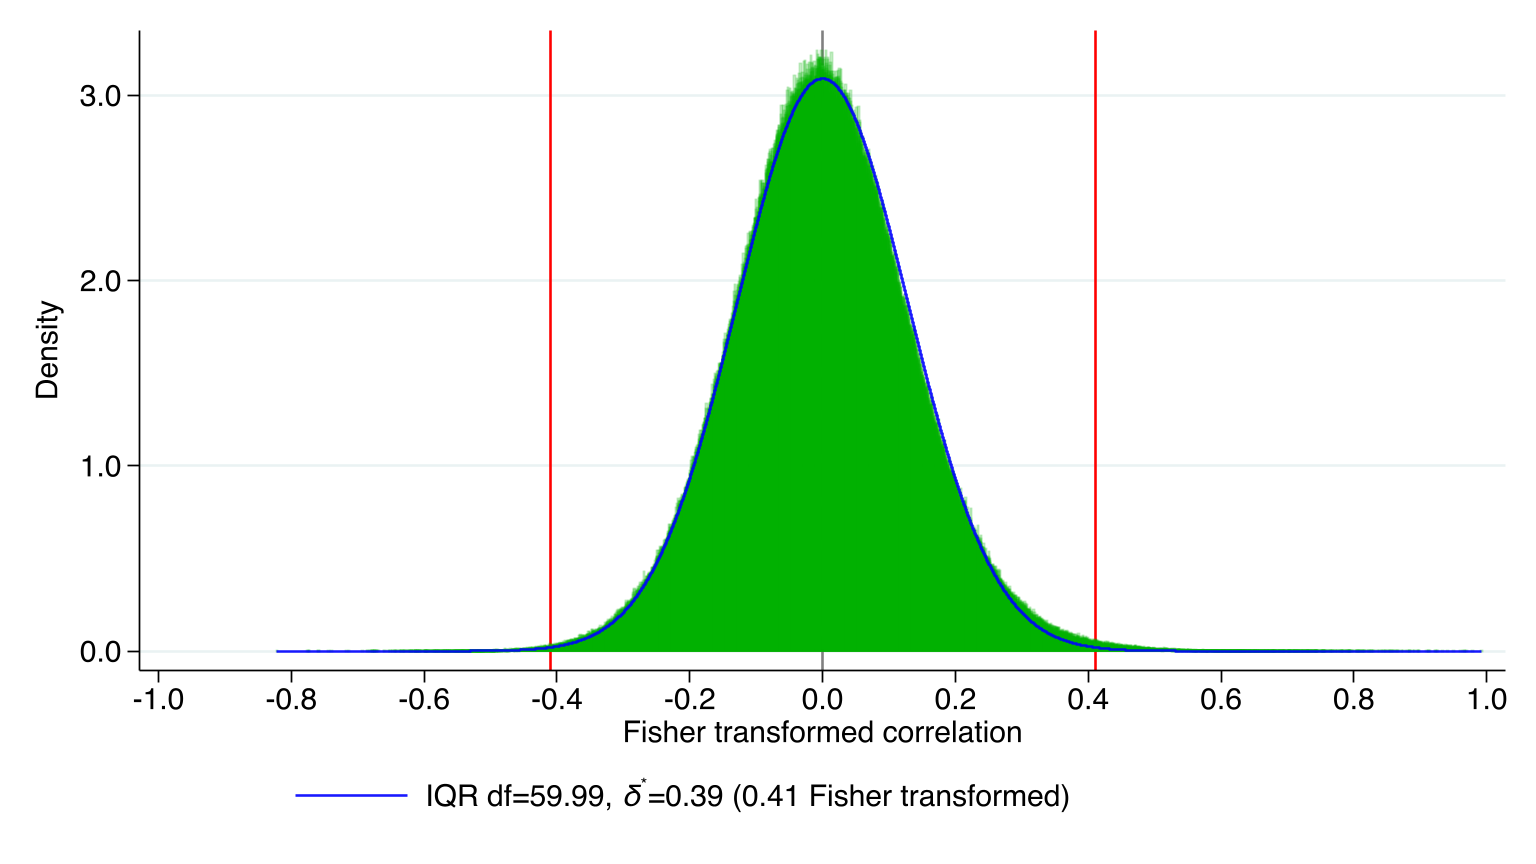
\includegraphics[width=\textwidth]{figures/_hist.png}
    \label{fisherCorr}
  \end{figure}

  \begin{figure}[H]
    \caption{Optimal Thresholding}
    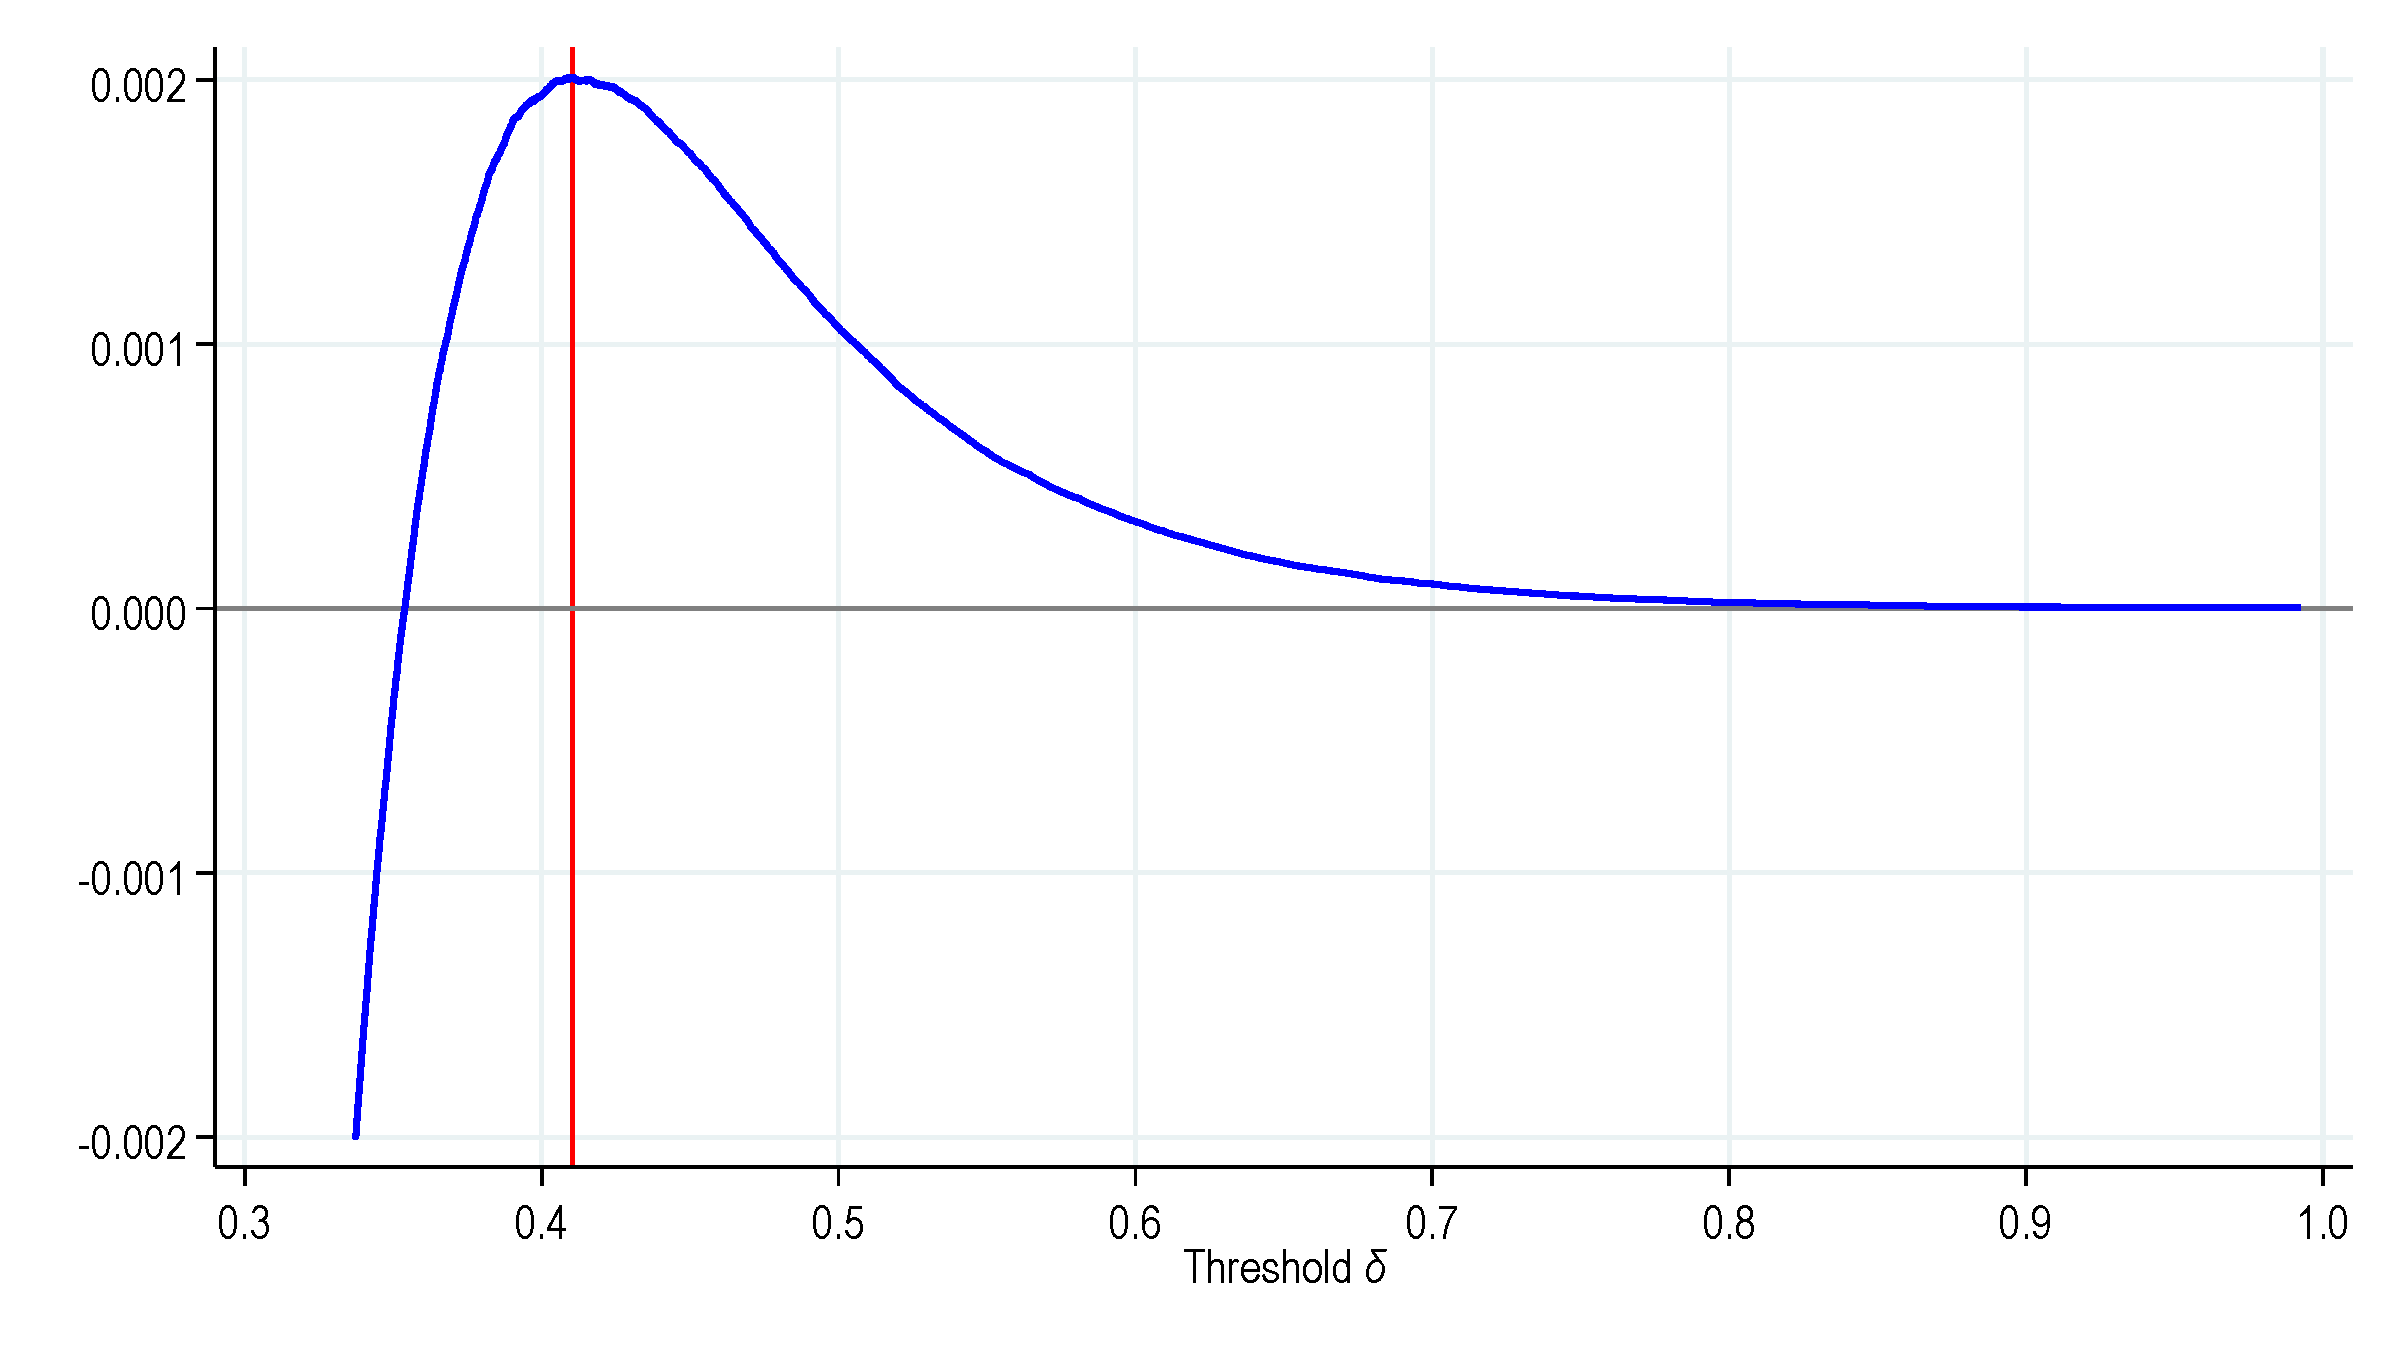
\includegraphics[width=\textwidth]{figures/_qt.pdf}
    \label{opThreshol}
  \end{figure}





\subsection{Alternative Models}
\paragraph{Instrumental Variables}
\texttt{tmo} can be used with instrumental–variables estimators. Using the same
cross sectional dataset, we estimate the effect of infant mortality on life expectancy
instrumenting \texttt{VST\_infmort\_d} with the median distance (in miles) to the
nearest emergency department, obstetrics department, and pediatric ICU. The \texttt{cmd()} option simply wraps the IV estimator you would normally use; its
contents follow the \emph{native} syntax of the chosen command. \texttt{tmo} is
compatible with \texttt{ivreg2}, \texttt{ivreghdfe}, and \texttt{ivregress}. The
option \texttt{x()} marks the endogenous/treatment variable whose coefficient’s
variance is to be adjusted, and \texttt{ylist()} supplies the auxiliary outcomes.

\begin{stlog}
\input{examples/Ivexample.tex.log}
\end{stlog}
The output mirrors the cross sectional case: the reported coefficient equals the
second–stage IV estimate from the underlying command, while the standard error is
TMO–adjusted; the lower block reports the optimal threshold,  
\paragraph{Panel Data}
Panel–ready data are available as \href{https://raw.githubusercontent.com/wjnkim/tmo/master/example/county_panel.dta}{\texttt{county\_panel.dta}} in the project repository on GitHub.
\smallskip

In panel settings, \texttt{tmo} incorporates the time dimension through the unit and time identifiers specified in \texttt{idvar()} and \texttt{timevar()}. The command treats \(\{i,t\}\) as a panel, reshapes the normalized residuals into an \(N\times T\) array, and computes cross location correlations using all periods. The sandwich matrix is then built from location pairs \((i,i^\prime)\) combined with time pairs, which increases computational cost; accordingly, the program prints progress messages such as ``\texttt{Computed X\% of sandwich}'' as it accumulates contributions by blocks.

\begin{stlog}
. tmo, cmd(reg EMN_farm EDU_publicenroll i.year i.stfips, cluster(fips)) ///
>     x(EDU_publicenroll) ylist(`ylist') i(fips) t(year)
Computed 0.00\% of sandwich
Computed 50.00\% of sandwich
{\smallskip}
Linear Regression with TMO                              Number of obs =  6,222
                                                        R-squared     = 0.3426
                                                        Adj R-squared = 0.3426
                                                        Root MSE      = 0.7683
{\smallskip}
\HLI{13}{\TOPT}\HLI{64}
    EMN_farm {\VBAR} Coefficient  Std. err.      t    P>|t|     [95\% conf. interval]
\HLI{13}{\PLUS}\HLI{64}
EDU_public{\tytilde}l {\VBAR}   .1355818   .0758575     1.79   0.074    -.0131541    .2843177
\HLI{13}{\BOTT}\HLI{64}
\HLI{79}
                                                                               
                                                   Optimal threshold      0.545
                                            \% of off-diag in SE est.      0.892
                              \% >= threshold (excl. clusters/Conley)      0.892
                                                          \# outcomes     63.000
                                                  Degrees of freedom     24.612
\HLI{79}

\end{stlog}
The output is analogous to the cross sectional case. The effective sample size increases because the data expand over time, and the optimal threshold may differ since correlations are constructed using the panel information. All reported fields keep the same interpretation as in the cross sectional setting.
\paragraph{Other routines}
Show that original estimator can be implemented by reg, reghdfe, areg.  Perhaps discuss time?  

\begin{stlog}
. timer clear
{\smallskip}
. timer on 1
{\smallskip}
. qui tmo, cmd(regress PIN_persincpc_d EDU_college_d i.stfips, r) ///
>     x(EDU_college_d) ylist(`ylist') i(fips)
{\smallskip}
. timer off 1
{\smallskip}
. 
. timer on 2
{\smallskip}
. qui tmo, cmd(reghdfe PIN_persincpc_d EDU_college_d, vce(r) abs(stfips)) ///
>     x(EDU_college_d) ylist(`ylist') i(fips)
{\smallskip}
. timer off 2
{\smallskip}
. 
. timer on 3
{\smallskip}
. qui tmo, cmd(areg PIN_persincpc_d EDU_college_d, r abs(stfips)) ///
>     x(EDU_college_d) ylist(`ylist') i(fips)
{\smallskip}
. timer off 3
{\smallskip}
. timer list
   1:      6.51 /        1 =       6.5150
   2:      7.91 /        1 =       7.9050
   3:      7.30 /        1 =       7.2990
{\smallskip}

\end{stlog}

\subsection{Alternative settings}
\subsubsection{Combining {\tt tmo} with other spatial dependence procedures}
% TODO: narrative -- show model with just clustered OLS; then just Conley or
% Muller and Watson; then just tmo (replicates original); then cluster+tmo and
% tmo+Muller-Watson. Consider a summary table with estout.
\begin{stlog}
. * (5a) cluster-robust baseline vs tmo with clustering
. reg PIN_persincpc_d EDU_college_d, cluster(stfips)
{\smallskip}
Linear regression                               Number of obs     =      3,060
                                                F(1, 47)          =      39.74
                                                Prob > F          =     0.0000
                                                R-squared         =     0.0708
                                                Root MSE          =     .16767
{\smallskip}
                                (Std. err. adjusted for 48 clusters in stfips)
\HLI{13}{\TOPT}\HLI{64}
             {\VBAR}               Robust
PIN_persin{\tytilde}d {\VBAR} Coefficient  std. err.      t    P>|t|     [95\% conf. interval]
\HLI{13}{\PLUS}\HLI{64}
EDU_colleg{\tytilde}d {\VBAR}   .2299788   .0364834     6.30   0.000     .1565835     .303374
       _cons {\VBAR}   1.934663   .0243343    79.50   0.000     1.885708    1.983617
\HLI{13}{\BOTT}\HLI{64}
{\smallskip}
. tmo, cmd(reg PIN_persincpc_d EDU_college_d, cluster(stfips)) ///
>     x(EDU_college_d) ylist(`ylist') i(fips)
{\smallskip}
Linear Regression with TMO                              Number of obs =  3,060
                                                        R-squared     = 0.0705
                                                        Adj R-squared = 0.0705
                                                        Root MSE      = 0.1677
{\smallskip}
\HLI{13}{\TOPT}\HLI{64}
PIN_persin{\tytilde}d {\VBAR} Coefficient  Std. err.      t    P>|t|     [95\% conf. interval]
\HLI{13}{\PLUS}\HLI{64}
EDU_colleg{\tytilde}d {\VBAR}   .2299788   .0381001     6.04   0.000     .1533312    .3066263
\HLI{13}{\BOTT}\HLI{64}
\HLI{79}
                                                                               
                                                   Optimal threshold      0.433
                                            \% of off-diag in SE est.    100.000
                              \% >= threshold (excl. clusters/Conley)    100.000
                                                          \# outcomes     90.000
                                                  Degrees of freedom     45.192
\HLI{79}
{\smallskip}
. 
. * (5b) tmo combined with SCPC (requires county centroids from maps data)
. preserve
{\smallskip}
. use "$SJ/data/maps/cb_2018_us_county_20m.dta", clear
{\smallskip}
. destring GEOID, replace
GEOID: all characters numeric; replaced as long
{\smallskip}
. tempfile maps
{\smallskip}
. save `maps'
file{\bftt{ /var/folders/l2/y38hz3_d2ndd62p9krlby05r0000gn/T//St98231.000002}} saved
    as .dta format
{\smallskip}
. restore
{\smallskip}
. 
. rename fips GEOID
{\smallskip}
. merge 1:1 GEOID using `maps', keep(3) nogen
{\smallskip}
    Result                      Number of obs
    \HLI{41}
    Not matched                             0
    Matched                             3,060  
    \HLI{41}
{\smallskip}
. // _CX: longitude ; _CY: latitude
. rename (_CY _CX) (s_1 s_2)
{\smallskip}
. // scpc reads s_* in physical variable order: force s_1 (lat) before s_2
. order s_1 s_2
{\smallskip}
. reg PIN_persincpc_d EDU_college_d, r
{\smallskip}
Linear regression                               Number of obs     =      3,060
                                                F(1, 3058)        =     168.81
                                                Prob > F          =     0.0000
                                                R-squared         =     0.0708
                                                Root MSE          =     .16767
{\smallskip}
\HLI{13}{\TOPT}\HLI{64}
             {\VBAR}               Robust
PIN_persin{\tytilde}d {\VBAR} Coefficient  std. err.      t    P>|t|     [95\% conf. interval]
\HLI{13}{\PLUS}\HLI{64}
EDU_colleg{\tytilde}d {\VBAR}   .2299788   .0177005    12.99   0.000     .1952727    .2646848
       _cons {\VBAR}   1.934663   .0089404   216.40   0.000     1.917133    1.952192
\HLI{13}{\BOTT}\HLI{64}
{\smallskip}
. scpc, latlong
found 3060 observations / clusters and 2-dimensional locations in s_*
Computing distances on surface of sphere treating s_1 as latitude and s_2 as lo
> ngitude
SCPC optimal q = 6 for maximal average pairwise correlation = 0.030
{\smallskip}
SCPC Inference for first 2 coefficients
{\smallskip}
               {\VBAR}      Coef     Std_Err     t      P>|t|    95\% Conf 
  \HLI{13}{\PLUS}\HLI{52}
  EDU_colleg{\tytilde}d {\VBAR}  .2299788    .0253915    9.06    0.000    .1625168 
         _cons {\VBAR}  1.934663    .0335045   57.74    0.000    1.843191 
{\smallskip}
               {\VBAR}  Interval  
  \HLI{13}{\PLUS}\HLI{12}
  EDU_colleg{\tytilde}d {\VBAR}  .2974407  
         _cons {\VBAR}  2.026134  
{\smallskip}
. rename (s_1 s_2) (_CY _CX)
{\smallskip}
. 
. tmo, cmd(regress PIN_persincpc_d EDU_college_d, r) ///
>     x(EDU_college_d) ylist(`ylist') i(GEOID) lat(_CY) lon(_CX) ///
>     scpc_cmd(reg PIN_persincpc_d EDU_college_d, r)
{\smallskip}
Linear Regression with TMO                              Number of obs =  3,060
                                                        R-squared     = 0.0705
                                                        Adj R-squared = 0.0705
                                                        Root MSE      = 0.1677
{\smallskip}
\HLI{13}{\TOPT}\HLI{64}
PIN_persin{\tytilde}d {\VBAR} Coefficient  Std. err.      t    P>|t|     [95\% conf. interval]
\HLI{13}{\PLUS}\HLI{64}
EDU_colleg{\tytilde}d {\VBAR}   .2299788   .0287255     8.01   0.000     .1736556    .2863019
\HLI{13}{\BOTT}\HLI{64}
\HLI{79}
                                                                               
                                                   Optimal threshold      0.433
                                            \% of off-diag in SE est.      0.667
                              \% >= threshold (excl. clusters/Conley)      0.667
                                                          \# outcomes     90.000
                                                  Degrees of freedom     45.192
\HLI{79}

\end{stlog}

\subsubsection{Cross-country data and the World Bank Databank}
Show wbopendata with cross-country.  Democracy and growth??

\section{Discussion and Conclusion}
\label{scn:discussion}

\clearpage

  \begin{Athanks}
    We are grateful to \ldots
    \end{Athanks}
    
    \bibliography{sj}
    
    \clearpage
    \begin{aboutauthors}
    Stefano DellaVigna is \ldots

    Guido Imbens is the Applied Econometrics Professor and Professor of Economics at Stanford Graduate School of Business.

    Woojin Kim is\ldots 
    
    David M. Ritzwoller is \ldots

    Damian Clarke is an Associate Professor at The Department of Economics of The Universidad de Chile and the University of Exeter, a Research Fellow at IZA and an Associate at the Millennium Institute for Market Imperfections and Public Policy.  
    

    Nicol\'as Par\'is is\ldots
    \end{aboutauthors}

\clearpage
\appendix
\section*{Appendix}



\begin{algorithm}[H]
\caption{Thresholding Multiple Outcomes (TMO)}
\label{alg:TMP}
\begin{algorithmic}[1]
\Require Outcome $Y_i^{(0)}$ and treatment $W_i$ for units $i=1,\ldots,n$
\Ensure Estimate of the variance of $\hat\tau^{(0)}$, the least-squares regression coefficient of $Y_i^{(0)}$ on $W_i$
\State Identify a collection of auxiliary outcomes $Y_i^{(1)},\ldots,Y_i^{(d)}$.
\State For each unit $i$ and outcome $j$, compute the normalized residuals $\hat\varepsilon_i^{(j)}$
\State For each pair of units $i\neq i'$, measure the correlation $\hat\rho_{i,i'}$
\State Approximate the null distribution of $\hat\rho_{i,i'}$ with $\mathrm{N}(0,\hat v)$, where $\hat v$ solves
\[
  \Phi_{\hat v}^{-1}(0.75)-\Phi_{\hat v}^{-1}(0.25)
  \;=\;
  G_{n,d}^{-1}(0.75)-G_{n,d}^{-1}(0.25),
\]
where $\Phi_v(\cdot)$ is the CDF of $\mathrm{N}(0,v)$, and $G_{n,d}(\cdot)$ is defined (paper)
\State Choose the threshold $\hat\delta^{\ast}$ by maximizing
\[
  \hat Q_{n,d}(\delta)
  \;=\;
  \bigl(\hat F_{n,d}(\delta)-F_0^{+}(\delta)\bigr) - F_0^{+}(\delta),
  \qquad \delta>0,
\]
where $F_0^{+}(\delta)=2\bigl(1-\Phi_{\hat v}(\cdot)\bigr)$ and $\hat F_{n,d}(\cdot)$ defined in (paper).
\State Collect the estimates
\[
\hat\sigma^{(0)}_{i,i'}(\hat\delta^{\ast}) =
\begin{cases}
 \hat\varepsilon_i^{(0)}\,\hat\varepsilon_{i'}^{(0)}, & i=i',\\[4pt]
 \hat\varepsilon_i^{(0)}\,\hat\varepsilon_{i'}^{(0)}\;\mathbb{I}\{\,|\hat\rho_{i,i'}|\ge \hat\delta^{\ast}\,\}, & i\neq i',
\end{cases}
\]
into the matrix $\hat\Sigma^{(0)}(\hat\delta^{\ast})$.
\State \textbf{Return} the variance estimate
\[
\hat V(\hat\delta^{\ast})
=
\bigl(W^{\top}W\bigr)^{-1}
\Bigl(W^{\top}\,\hat\Sigma^{(0)}(\hat\delta^{\ast})\,W\Bigr)
\bigl(W^{\top}W\bigr)^{-1}.
\]
\end{algorithmic}
\end{algorithm}
    
    \end{document}
